
\iffalse

\begin{table*}[h]
	\centering
	\resizebox{\linewidth}{!}{%
		\begin{tabular}{l|l|l|l|l|l|l|l|l|l|l|l|l|l|l|l|}
			\cline{2-16}
			& \multicolumn{3}{c|}{\textbf{JAVA}} & \multicolumn{3}{c|}{\textbf{JS}} & \multicolumn{3}{c|}{\textbf{CPP}} & \multicolumn{3}{c|}{\textbf{CS}} & \multicolumn{3}{c|}{\textbf{PHP}}                                                 \\ \cline{2-16} 
			& Avg    & Min    & Max     & Avg    & Min   & Max    & Avg    & Min    & Max    & Avg    & Min   & Max    & Avg   & Min   & Max \\ \hhline{|=|=|=|=|=|=|=|=|=|=|=|=|=|=|=|=|}
			\multicolumn{1}{|l|}{Color}   & 2.72   & 0,69   & 28,58   & 1,67   & 0,52  & 16,66  & 3,52   & 0,37   & 48,31  & 3,81   & 0,52  & 45,97  & 23,16  & 0,61  &  279,27  \\ \hline
			\multicolumn{1}{|l|}{Core}    & 9,25   & 0,57   & 8,71    & 15,01   & 0,51  & 14,01  & 14,49   & 0,42   & 8,11   & 24,07   & 0,50  & 21,60  &  1238,49  & 0,47  &  2479,07 \\ \hline
			\multicolumn{1}{|l|}{Hxmath}  & 1,62   & 0,66   & 3,38    & 1,1    & 0,54  & 2,04   & 0,81   & 0,39   & 1,42   & 1,64   & 0,56  & 4,01   &  26,53  & 1,06  &  73,44   \\ \hline
			\multicolumn{1}{|l|}{Format}  & 2,19   & 0,71   & 5,03    & 2,23   & 0,60  & 5,402  & 2,57   & 0,37   & 7,67   & 4,97   & 0,54  & 12,38  &  93,53  & 1,11  &  220,75  \\ \hline
			\multicolumn{1}{|l|}{Promise} & 0,89   & 0,63   & 1,72    & 1,44   & 0,54  & 2,09   & 0,69   & 0,39   & 1,12   & 0,99   & 0,48  & 1,71   &  11,96  & 1,13  &  31,18   \\ \hline
			\multicolumn{1}{|l|}{Culture} & 0,64   & 0,55   & 0,82    & 0,50   & 0,46  & 0,57   & 0,44   & 0,37   & 0,62   & 0,50   & 0,43  & 0,65   & 1,46                           & 0,61  & 3,79                            \\ \hline
			\multicolumn{1}{|l|}{Math}    & 5,26   & 0,98   & 12,51   & 1,66   & 0,75  & 3.10   & 6,30   & 0,93   & 16,29  & 5,75   & 0,94  & 14,14  & 523,17 & 55,45 &  1448,9  \\ \hline
		\end{tabular}%
	}
	\caption{Execution time stats}
	\label{my-label}
\end{table*}
% Please add the following required packages to your document preamble:
% \usepackage[table,xcdraw]{xcolor}
% If you use beamer only pass "xcolor=table" option, i.e. \documentclass[xcolor=table]{beamer}


\begin{table*}[h]
	\centering
	
	\resizebox{\linewidth}{!}{%
		\begin{tabular}{l|l|l|l|l|l|l|l|l|l|l|l|l|l|l|l|}
			\cline{2-16}
			& \multicolumn{3}{c|}{\textbf{JAVA}} & \multicolumn{3}{c|}{\textbf{JS}} & \multicolumn{3}{c|}{\textbf{CPP}} & \multicolumn{3}{c|}{\textbf{CS}} & \multicolumn{3}{c|}{\textbf{PHP}}                                                 \\ \cline{2-16} 
			& Avg    & Min    & Max     & Avg    & Min   & Max    & Avg    & Min    & Max    & Avg    & Min   & Max    & Avg   & Min   & Max \\ \hhline{|=|=|=|=|=|=|=|=|=|=|=|=|=|=|=|=|}
			\multicolumn{1}{|l|}{Color}   & 115,98  & 0,53  & 1362,55 & 62,33   & 0,70 & 900,70 & 169,90  & 0,16 & 2275,49 & 87,51   & 0,42 & 1283,3 & 173,69  & 0,81   & 2189,85 \\ \hline
			\multicolumn{1}{|l|}{Core}    & 55,32   & 0,52  & 1057,32 & 12,85    & 0,64 & 59,96  & 21,19    & 0,29 & 35,97   & 16,66    & 0,59 & 42,92  & 111,10    & 0,46   & 32,91   \\ \hline
			\multicolumn{1}{|l|}{Hxmath}  & 121,47  & 0,70  & 389,72  & 37,23   & 1,37 & 111,68 & 96,15   & 1,20 & 296,43  & 50,19   & 0,81 & 156,40 & 472,26  & 1,11   & 1192,98 \\ \hline
			\multicolumn{1}{|l|}{Format}  & 214,04  & 0,67  & 685,90  & 38,93   & 2,42 & 92,34  & 70,29   & 1,12 & 204,85  & 31,11   & 1,08 & 69,16  & 177,17  & 0,58   & 385,11  \\ \hline
			\multicolumn{1}{|l|}{Promise} & 32,85   & 1,23  & 128,29  & 31,65   & 0,54 & 55,29  & 0,93    & 0,45 & 1,73    & 12,85   & 0,87 & 34,49  & 57,96   & 0,65   & 134,20  \\ \hline
			\multicolumn{1}{|l|}{Culture} & 2,20    & 1,15  & 4,04    & 1,12    & 0,70 & 1,59   & 1,68    & 1,35 & 2,02    & 3,34    & 0,55 & 11,20  & 10,11   & 1,11   & 36,32   \\ \hline
			\multicolumn{1}{|l|}{Math}    & 353,18  & 1,21  & 831,44  & 165,71  & 0,93 & 493,66 & 597,02  & 1,61 & 1492,97 & 312,37  & 3,37 & 806,33 & 1448,45 & 626,83 & 3088,15 \\ \hline
		\end{tabular}%
	}
	\caption{Memory stats}
	\label{my-label}
\end{table*}


\begin{table}[]
	\centering
	
	\begin{tabular}{|l|l|l|l|l|}
		\hline
		& \textbf{JAVA} & \textbf{CPP}  & \textbf{CS}   & \textbf{PHP}   \\ \hhline{|=|=|=|=|=|}
		Color   & 1,86 & 2,72 & 1,40 & 2,78  \\ \hline
		Core    & 4.30 & 1.64 & 1,29 & 8,64  \\ \hline
		Hxmath  & 3,26 & 2,58 & 1,34 & 12,68 \\ \hline
		Format  & 5,49 & 1,80 & 0,79 & 4,55  \\ \hline
		Promise & 1,03 & 0,02 & 0,40 & 1,83  \\ \hline
		Culture & 1,95 & 1,49 & 2,96 & 8,96  \\ \hline
		Math    & 2,13 & 3,60 & 1,88 & 8,74  \\ \hline
	\end{tabular}
	\caption{Average memory usage compared to JS version}
	\label{my-label}
\end{table}
\begin{table}[]
	\centering
	
	\begin{tabular}{|l|l|l|l|l|}
		\hline
		& \textbf{JAVA} & \textbf{CPP}  & \textbf{CS}   & \textbf{PHP}    \\ 	\hhline{|=|=|=|=|=|}
		Color   & 1,63 & 2,10 & 2,28 & 13,86  \\ \hline
		Core    & 0,65 & 1,03 & 1,71 & 88,34  \\ \hline
		Hxmath  & 1,47 & 0,73 & 1,49 & 24,11  \\ \hline
		Format  & 0,97 & 1,15 & 2,22 & 41,79  \\ \hline
		Promise & 0,61 & 0,47 & 0,68 & 8,27   \\ \hline
		Culture & 1,27 & 0,87 & 0,99 & 2,89   \\ \hline
		Math    & 3,16 & 3,79 & 3,46 & 314,65 \\ \hline
	\end{tabular}
	\caption{Average execution time compared to JS version}
	\label{my-label}
\end{table}

\begin{table}[]
	\centering
	
	\begin{tabular}{|l|l||l|}
		\hline
		& \multicolumn{1}{c||}{\begin{tabular}[c]{@{}c@{}}\textbf{Average}\\ \textbf{speed}\end{tabular}} & \begin{tabular}[c]{@{}l@{}}\textbf{Average}\\ \textbf{memory}\end{tabular} \\ 	\hhline{|=|=|=|}
		JAVA & 3,22                                                                         & 127,86                                                   \\ \hline
		JS   & 3,23                                                                         & 49,97                                                    \\ \hline
		CPP  & 4,12                                                                         & 136,74                                                   \\ \hline
		CS   & 5,96                                                                         & 73,43                                                    \\ \hline
		PHP  & 274,04                                                                       & 350,10                                                   \\ \hline
	\end{tabular}
	\caption{Average memory usage and execution speed per target language}
	\label{my-label}
\end{table}



\begin{figure}[h]
	\centering
	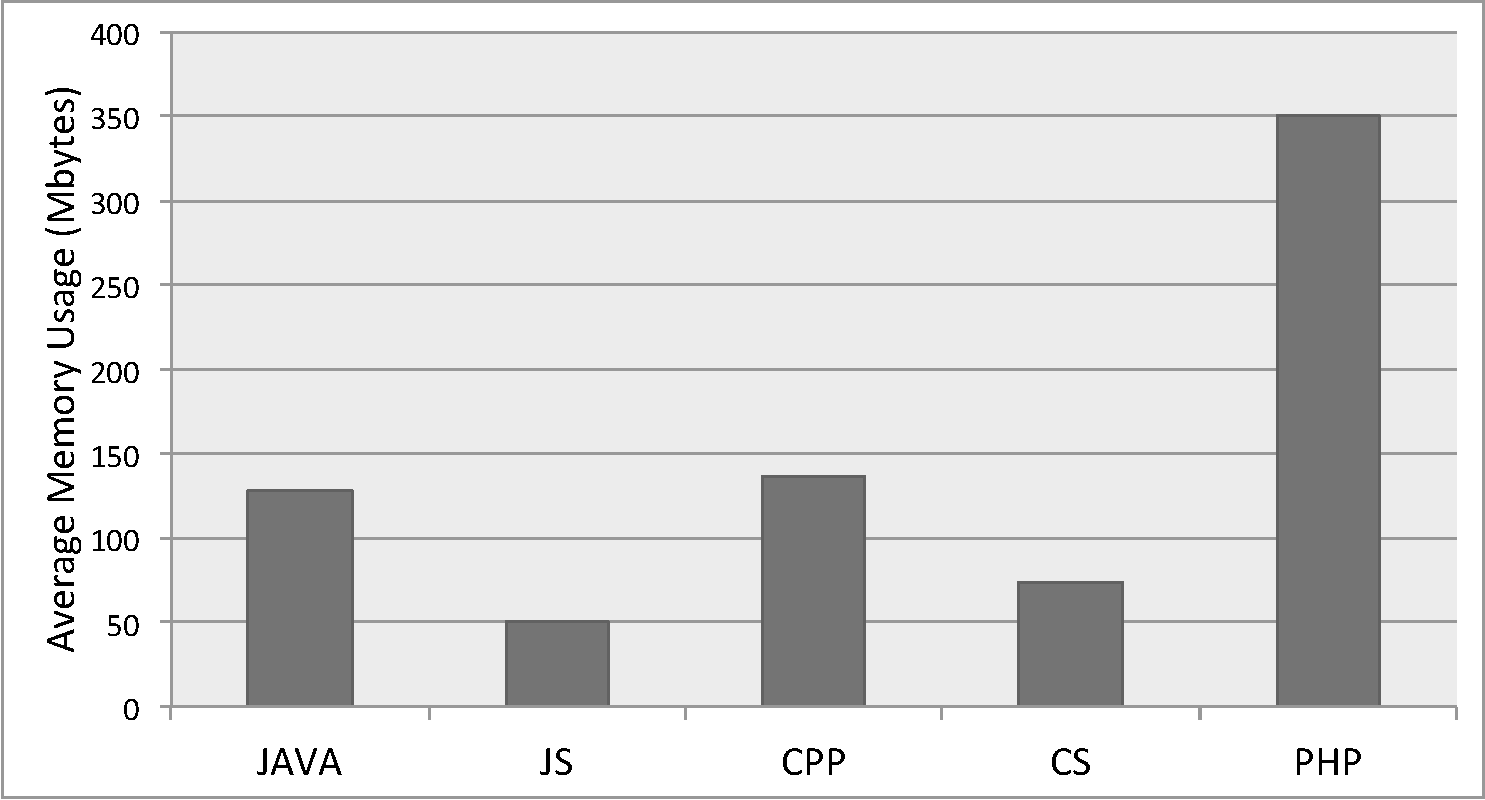
\includegraphics[width=1\linewidth]{Ressources/avgmem.pdf}
	\caption{Comparison of average memory consumption and execution time of FFmpeg containers compiled with standard GCC optimization options}
\end{figure}
\begin{figure}[h]
	\centering
	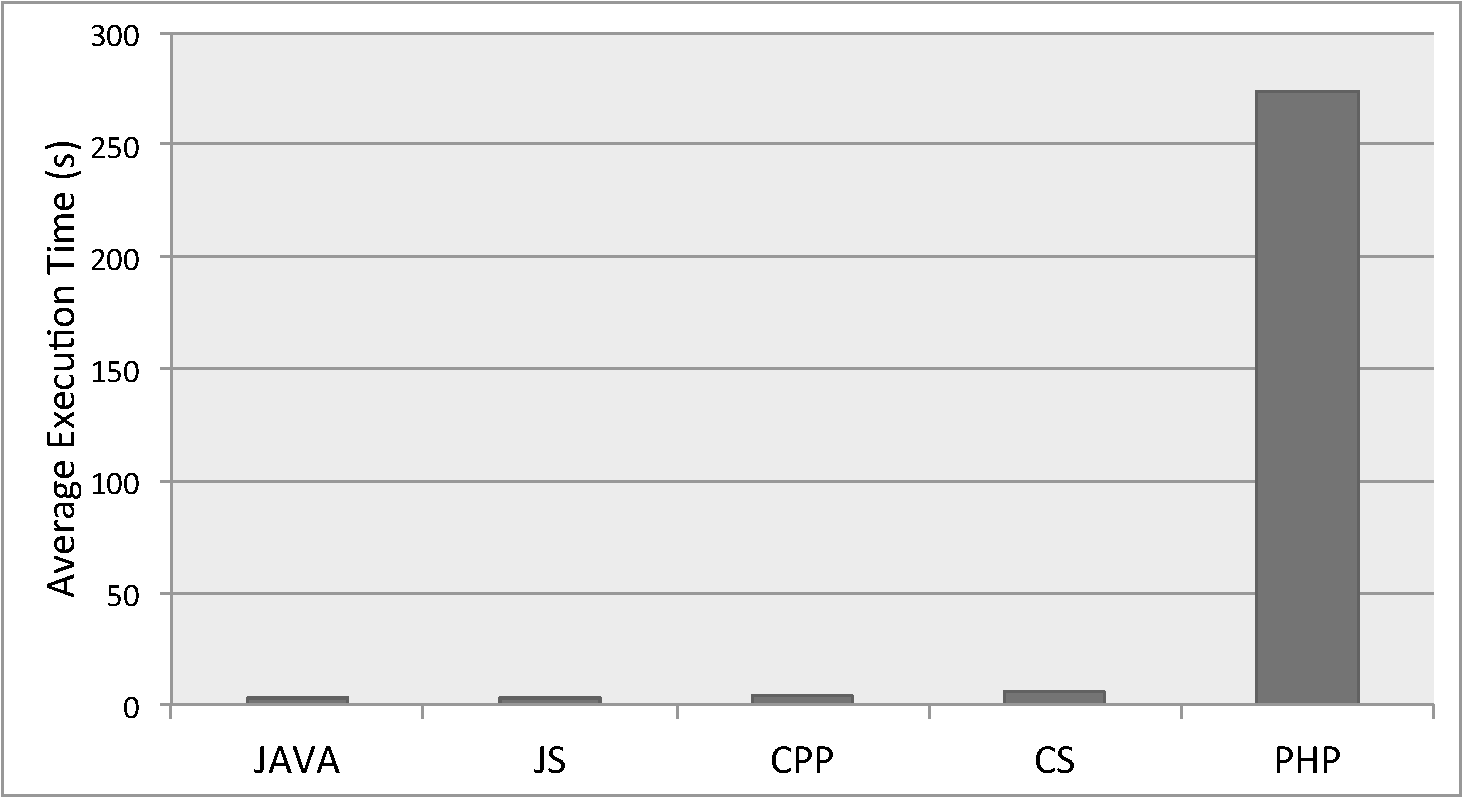
\includegraphics[width=1\linewidth]{Ressources/avgtime.pdf}
	\caption{Comparison of average memory consumption and execution time of FFmpeg containers compiled with standard GCC optimization options}
\end{figure}
\fi